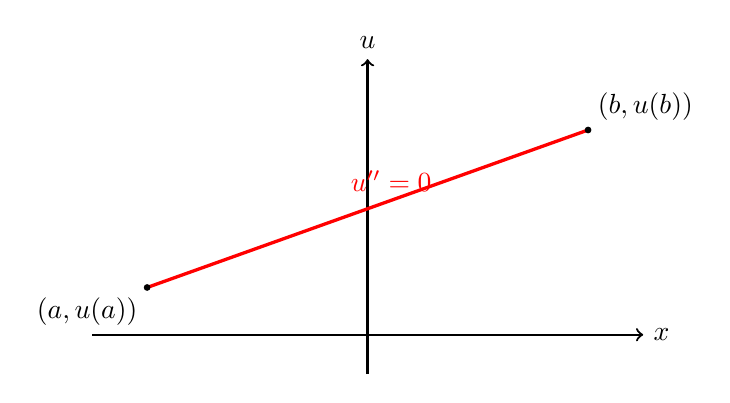
\begin{tikzpicture}[scale=1.0]
  % axes
  \draw[->, thick] (-3.5,0) -- (3.5,0) node[right] {$x$};
  \draw[->, thick] (0,-0.5) -- (0,3.5) node[above] {$u$};

  % endpoints
  \coordinate (A) at (-2.8, 0.6);
  \coordinate (B) at (2.8, 2.6);

  % straight line
  \draw[red, very thick] (A) -- (B);
  \node[red] at (0.3, 1.95) {$u''=0$};

  % endpoints
  \filldraw (A) circle (1pt) node[below left] {$(a,u(a))$};
  \filldraw (B) circle (1pt) node[above right] {$(b,u(b))$};
\end{tikzpicture}